\section{Implementation}

PQVRS is open source (10K lines of code across C++, Matlab, Java, and python) and can be accessed at \cite{github}. Implementation of PQVRS is shown in Fig. \ref{implementation}. Compared with traditional video streaming system, several modules are newly added or modified, which are highlighted by pink color.

\begin{figure}
  \centering
  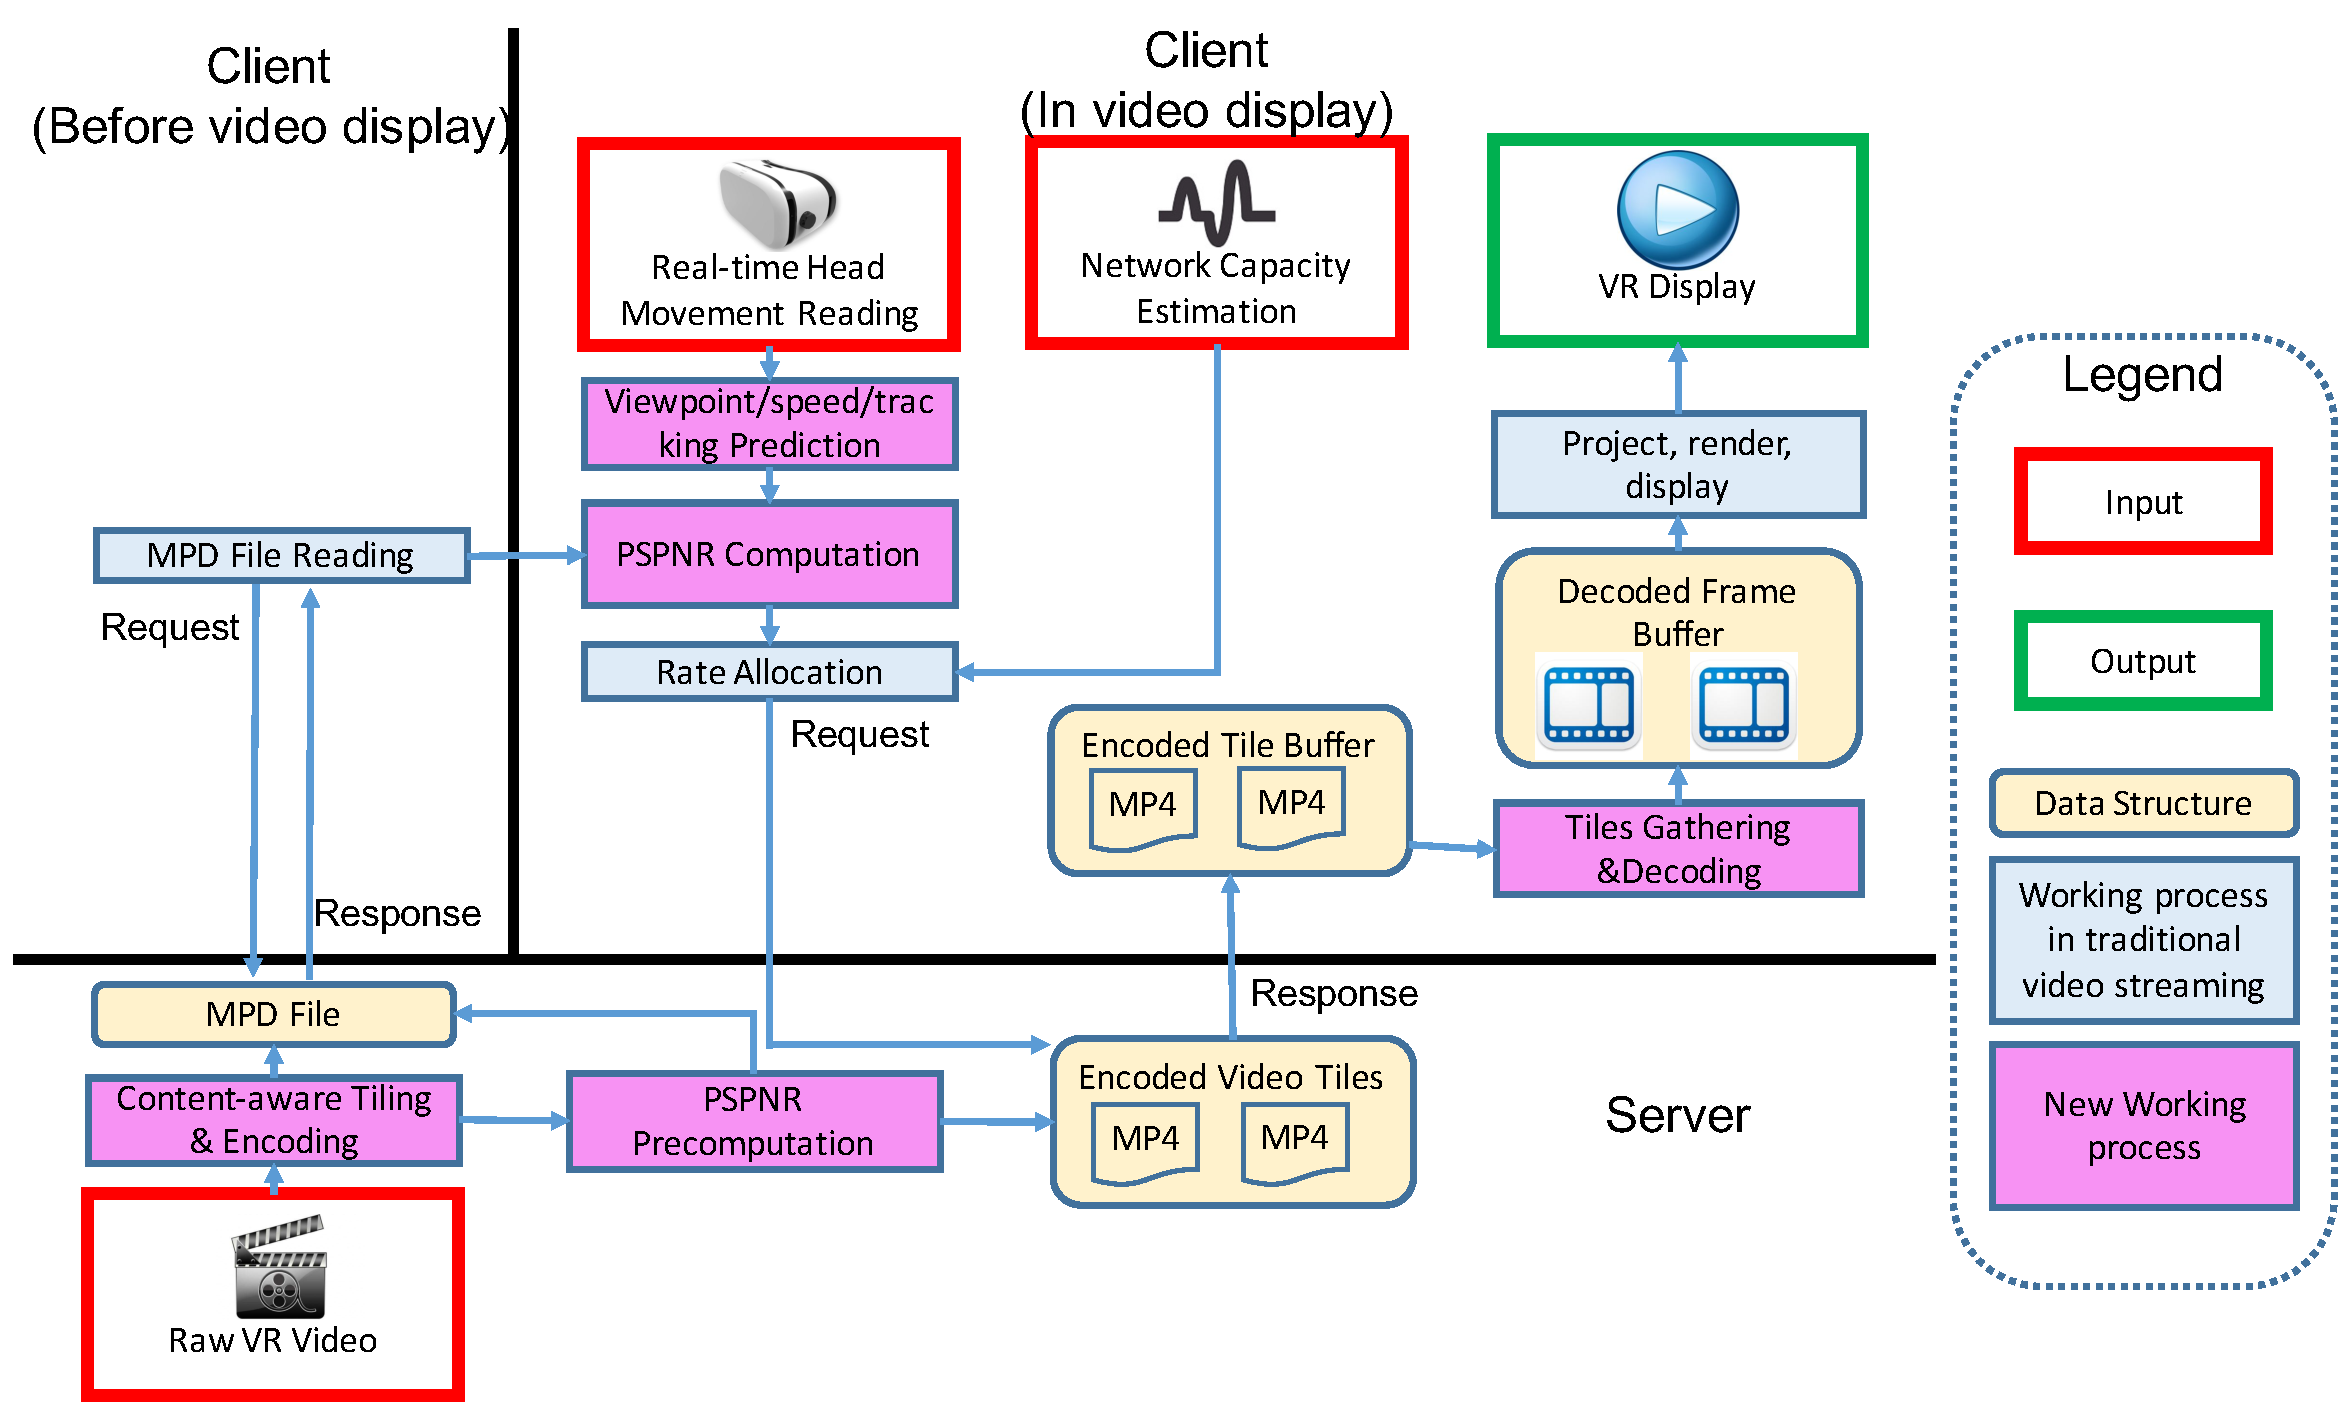
\includegraphics[width=3.5in]{images/implementation.pdf}
  \caption{Workflow of PQVRS.}
  \label{implementation}
  \end{figure}

\subsection{Server-Side}

\textbf{Content-Aware Tiling / Encoding:} Based on our tiling algorithm described in Sec. 5, we cut each video segment into $N = 72$ rectangular tiles with different size. Each tile is encoded independently. The information of tiling result is packeted into MPD file so that client is aware of how each segment is cut. In addition, to prevent client-side stalling, we encode the lowest quality version of whole video without tiling, called "Base Layer".\cite{buffer} Then client-side can set up a 30s buffer for Base Layer and 5s buffer for tiles with high quality. \cite{buffer} This large-size Base Layer buffer significantly reduces stalling, compared with only a 5s buffer for tiles.

For each video segment, we first transfer the Base Layer to client, and then transfer tiles only in user's viewport with corresponding quality. This can significantly reduce the number of tiles decoded on client-side (from 72 to around 12 per video segment), thus make PQVRS applicable on real-world devices.

\textbf{PSPNR Precomputation:} Based on equation (x), server tries to compute PSPNR of each tile for 5 different BJNDs, then packet the result into MPD file. Compared with video content, size of this additional information is negligible.

\subsection{Client-Side}

\textbf{Viewpoint / Speed / Tracking prediction:} In our system, viewpoint prediction is achieved by linear regression because of its efficiency and robustness. According to result of viewpoint prediction, we can estimate user's viewpoint moving speed by differentiating adjacent user viewpoints. Moreover, since we have analyzed object traces of video on server-side by YOLO \cite{yolo} and deliver the brief description to client-side, client-side can match the predictive viewpoint traces and object traces in order to predict if user is going to tracking an object.

\textbf{PSPNR Computation:} On client-side, based on our viewpoint / speed / tracking prediction, the value of BJND can be obtained by equation (x). Then client read MPD file to get the PSPNR results with different BJNDs, and choose the one with the nearest BJND.

\textbf{Tiles Gathering \& Decoding:} For each video segment, client first decode the Base Layer. For tiles in user's viewport, we set up a multi-process decoder based on ffmpeg, and set up a buffer to cache the decoded frames of tiles to be played in the future. Specifically, the decoding scheduler dynamically selects a received tile and sends it to an idle decoder. The decoded frames are not necessarily consumed right away; instead they can be stored in the buffer residing in the video memory. When a cached frame is needed during the playback, its corresponding tiles are fed into GPU, then then mapping them from 2D to 3D for rendering on Head-Mounted Device.